% --------------------------------------------------------------
% This is all preamble stuff that you don't have to worry about.
% Head down to where it says "Start here"
% --------------------------------------------------------------

\documentclass[12pt]{article}

\usepackage[margin=1in]{geometry}
\usepackage{amsmath,amsthm,amssymb}
\usepackage{tikz}
\usepackage{mathtools}

\usepackage{graphicx}
\graphicspath{ {images/} }

\DeclarePairedDelimiter{\ceil}{\lceil}{\rceil}

\usetikzlibrary{arrows}

\newcommand{\N}{\mathbb{N}}
\newcommand{\Z}{\mathbb{Z}}

\newenvironment{theorem}[2][Theorem]{\begin{trivlist}
\item[\hskip \labelsep {\bfseries #1}\hskip \labelsep {\bfseries #2.}]}{\end{trivlist}}
\newenvironment{lemma}[2][Lemma]{\begin{trivlist}
\item[\hskip \labelsep {\bfseries #1}\hskip \labelsep {\bfseries #2.}]}{\end{trivlist}}
\newenvironment{exercise}[2][Exercise]{\begin{trivlist}
\item[\hskip \labelsep {\bfseries #1}\hskip \labelsep {\bfseries #2.}]}{\end{trivlist}}
\newenvironment{question}[2][Question]{\begin{trivlist}
\item[\hskip \labelsep {\bfseries #1}\hskip \labelsep {\bfseries #2.}]}{\end{trivlist}}
\newenvironment{proposition}[2][Proposition]{\begin{trivlist}
\item[\hskip \labelsep {\bfseries #1}\hskip \labelsep {\bfseries #2.}]}{\end{trivlist}}
\newenvironment{corollary}[2][Corollary]{\begin{trivlist}
\item[\hskip \labelsep {\bfseries #1}\hskip \labelsep {\bfseries #2.}]}{\end{trivlist}}

\begin{document}

% --------------------------------------------------------------
%                         Start here
% --------------------------------------------------------------

%\renewcommand{\qedsymbol}{\filledbox}

\title{Homework 5}%replace X with the appropriate number
\author{Dustin Lambright - dalambri \\ Aseem Raina - araina \\ Bihan Zhang - bzhang28 \\ Anshul Fadnavis - asfadnav\\
%replace with your name
CSC 565 - Graph Theory} %if necessary, replace with your course title

\maketitle


\begin{question}{1}
Problem 4.1.8, text. For each $k$, which graphs are $k$-connected? Which are $k$-edge connected?
\end{question}

\noindent

\begin{center}
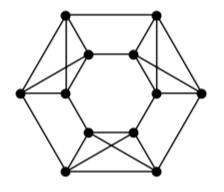
\includegraphics[scale=.65]{hexagon}

\begin{tabular}{l}
$\kappa$: 4 \\
$\kappa$':4 \\
$\delta$: 4 \\

\end{tabular} \\
\begin{tabular}{|c|c|c|}\hline
k & k-connected & k-edge connected \\ \hline
1 & Yes & Yes \\ \hline
2 & Yes & Yes \\ \hline
3 & Yes & Yes \\ \hline
4 & Yes & Yes \\ \hline
$\geq$5 & No & No \\ \hline
\end{tabular}



\clearpage
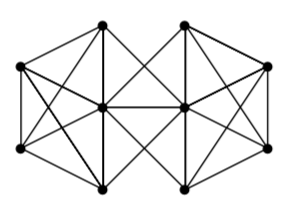
\includegraphics[scale=.65]{bigOne}\\

$\kappa$: 2 \\
$\kappa$':4 \\
$\delta$: 4 \\

\begin{tabular}{|c|c|c|}\hline
k & k-connected & k-edge connected \\ \hline
1 & Yes & Yes \\ \hline
2 & Yes & Yes \\ \hline
3 & No & Yes \\ \hline
4 & No & Yes \\ \hline
$\geq$5 & No & No \\ \hline
\end{tabular}


\end{center}


\begin{question}{2}
For $k \leq n - 1$, prove that every simple $n$-vertex graph $G$ with $\delta(G) \geq (n+k-2)/2$ is $k$-connected.
\end{question}


\begin{question}{3}

($!$) Prove that the symmetric difference of two different edge cuts is an edge cut. (Hint: Draw a picture illustrating the two edge cuts and use it to guide the proof.)

Let A be the edge cut of  $[X,\bar{X}]$ and B be the edge cut of $[Y,\bar{Y}]$. The symmetric difference of $A \Delta B$ is $(X \cup Y) - (X \cap Y)$. 

This can be shown in 4 cases: \\
1. An edge in A but not in B.

	In this case $e \in (X \cup Y)$ and $e \notin (X \cap Y)$ Thus $e \in \delta((X \cup Y) - (X \cap Y))$\\	
2. An edge in B but not in A

	In this case $e \in (X \cup Y)$ and $e \notin (X \cap Y)$ Thus $e \in \delta((X \cup Y) - (X \cap Y))$\\	
3. An edge in A and in B

	In this case $e \in (X \cup Y)$ and $e \in (X \cap Y)$ Thus $e \notin \delta((X \cup Y) - (X \cap Y))$\\	
4. An edge not in A or B

	In this case $e \notin (X \cup Y)$ and $e \notin (X \cap Y)$ Thus $e \notin \delta((X \cup Y) - (X \cap Y))$\\	
	
So $[(X \cup Y) - (X \cap Y), \overline{(X \cup Y) - (X \cap Y)}]$ is the resulting symmetric difference.

	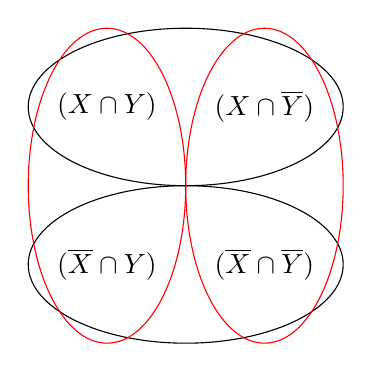
\begin{tikzpicture}
	\draw (0,0) ellipse (2cm and 1cm);
	\draw (0,2) ellipse (2cm and 1cm);
	\draw[red] (-1,1) ellipse (1cm and 2cm);
	\draw[red] (1,1) ellipse (1cm and 2cm);
	\node at (-1,2){$(X \cap Y)$};
	\node at (1,0){$(\overline{X} \cap \overline{Y})$};
	\node at (1,2){$(X \cap \overline{Y})$};
	\node at (-1,0){$(\overline{X} \cap Y)$};
	\end{tikzpicture}
	
\end{question}

\begin{question}{4}
($-$) Let $G$ be the simple graph with vertex set \{1...11\} defined by $i \leftrightarrow j$ if and only if $i, j$ have a common factor bigger than 1.  Determine the blocks of $G$.
\begin{align*}
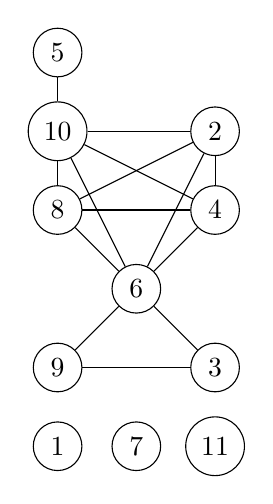
\begin{tikzpicture}
\node[shape=circle,draw=black] (A) at (0,5) {5};
\node[shape=circle,draw=black] (B) at (0,4) {10};
\node[shape=circle,draw=black] (C) at (2,4) {2};
\node[shape=circle,draw=black] (D) at (0,3) {8};
\node[shape=circle,draw=black] (E) at (2,3) {4};
\node[shape=circle,draw=black] (F) at (1,2) {6};
\node[shape=circle,draw=black] (G) at (0,1) {9};
\node[shape=circle,draw=black] (H) at (2,1) {3};
\node[shape=circle,draw=black] (I) at (0,0) {1};
\node[shape=circle,draw=black] (I) at (1,0) {7};
\node[shape=circle,draw=black] (I) at (2,0) {11};
\path [] (A) edge node[left] {} (B);
\path [] (B) edge node[left] {} (C);
\path [] (B) edge node[left] {} (D);
\path [] (B) edge node[left] {} (E);
\path [] (B) edge node[left] {} (F);
\path [] (C) edge node[left] {} (D);
\path [] (C) edge node[left] {} (E);
\path [] (C) edge node[left] {} (F);
\path [] (D) edge node[left] {} (E);
\path [] (D) edge node[left] {} (F);
\path [] (E) edge node[left] {} (F);
\path [] (F) edge node[left] {} (G);
\path [] (F) edge node[left] {} (H);
\path [] (G) edge node[left] {} (H);
\end{tikzpicture}
\end{align*}

The blocks are: $V(5, 10) $, $V(6,9,3)$, $V(1)$, $V(7)$, $V(11)$, $V(10,2,4,6,8)$
\end{question}

\begin{question}{5}
	Give a formula for the number of spanning trees of G in terms of the number of spanning trees of its blocks.	\\
	Let G be a connected graph that can be decomposed into $n$ Blocks $B_n$. The number of spanning trees in G is the product of the number of spanning trees in all it's blocks: \\

	$\tau(G) = \prod_{i=1}^{n}\tau(B_i)$\\
	This is because:\\
	- The graph can be decomposed into its blocks\\
	- Any combination of spanning trees of all blocks will still leave the resultant graph (now a spanning tree) connected, as long as the original graph is connected.
\end{question}

\begin{question}{6}
($-$) Determine $\kappa(u,v)$ and $\kappa`(u,v)$ in the graph drawn below. (Hint: Use the dual problems to give short proofs of optimality)

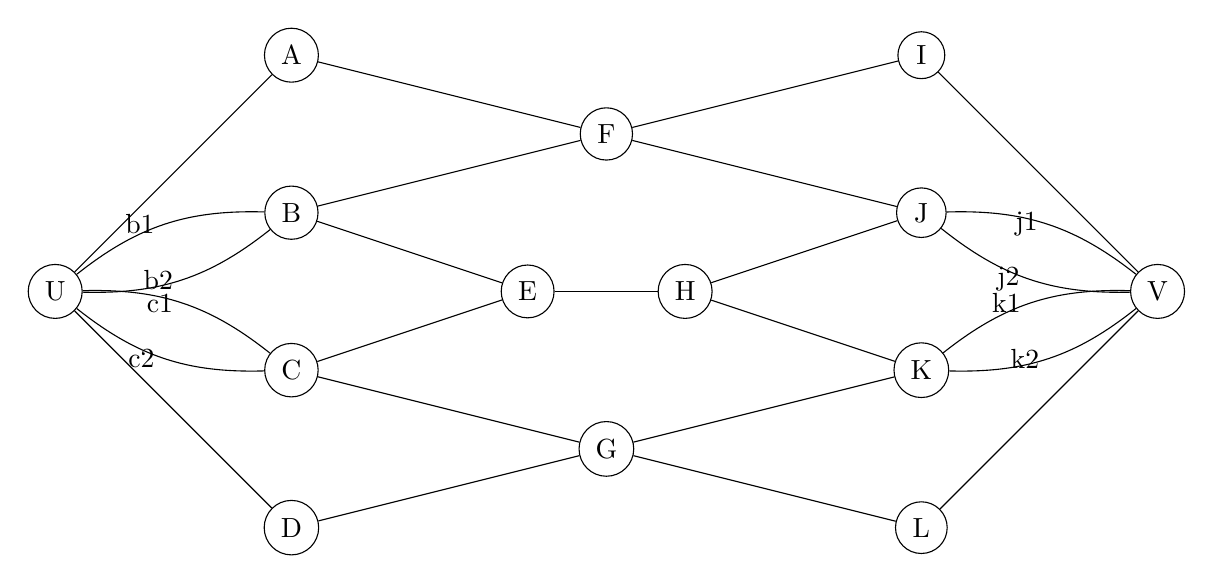
\begin{tikzpicture}
\tikzset{edge/.style = {->,> = latex'}}

\node[shape=circle,draw=black] (U) at (0,3) {U};
\node[shape=circle,draw=black] (A) at (3,6) {A};
\node[shape=circle,draw=black] (B) at (3,4) {B};
\node[shape=circle,draw=black] (C) at (3,2) {C};
\node[shape=circle,draw=black] (D) at (3,0) {D};
\node[shape=circle,draw=black] (E) at (6,3) {E};
\node[shape=circle,draw=black] (F) at (7,5) {F};
\node[shape=circle,draw=black] (G) at (7,1) {G};
\node[shape=circle,draw=black] (H) at (8,3) {H};
\node[shape=circle,draw=black] (I) at (11,6) {I};
\node[shape=circle,draw=black] (J) at (11,4) {J};
\node[shape=circle,draw=black] (K) at (11,2) {K};
\node[shape=circle,draw=black] (L) at (11,0) {L};
\node[shape=circle,draw=black] (V) at (14,3) {V};

\path [] (U) edge node[left] {} (A);
\path [] (U) edge [bend left=20] node[left] {b1} (B);
\path [] (U) edge [bend right=20] node[left] {b2} (B);
\path [] (U) edge [bend left=20] node[left] {c1} (C);
\path [] (U) edge [bend right=20] node[left] {c2} (C);
\path [] (U) edge node[left] {} (D);
\path [] (A) edge node[left] {} (F);
\path [] (B) edge node[left] {} (F);
\path [] (B) edge node[left] {} (E);
\path [] (C) edge node[left] {} (E);
\path [] (C) edge node[left] {} (G);
\path [] (D) edge node[left] {} (G);
\path [] (E) edge node[left] {} (H);
\path [] (F) edge node[left] {} (I);
\path [] (F) edge node[left] {} (J);
\path [] (G) edge node[left] {} (K);
\path [] (G) edge node[left] {} (L);
\path [] (H) edge node[left] {} (J);
\path [] (H) edge node[left] {} (K);
\path [] (I) edge node[left] {} (V);
\path [] (J) edge [bend left=20] node[left] {j1} (V);
\path [] (J) edge [bend right=20] node[left] {j2} (V);
\path [] (K) edge [bend left=20] node[left] {k1} (V);
\path [] (K) edge [bend right=20] node[left] {k2} (V);
\path [] (L) edge node[left] {} (V);
\end{tikzpicture}
\\
For the given graph (with nodes and some edges annotated for convenience):\\
\\
$\kappa(u, v) = 3$\\
For proof of optimality, we could use the duality:\\
$\kappa(u, v) = $ number of vertex-disjoint paths between $u$ and $v$, which are the following:\\
$u-A-F-I-v$\\
$u-B-E-H-J-v$\\
$u-C-G-K-v$\\
In other words, all $u-v$ paths must contain at least one of F, E or G.\\
\\
$\kappa'(u, v) = 5$\\
For proof of optimality, we could use the duality:\\
$\kappa'(u, v) = $ number of edge-disjoint paths between $u$ and $v$, which are the following:\\
$uA-AF-FI-Iv$\\
$b1-BF-FJ-j1$\\
$b2-BE-EH-HJ-j2$\\
$c1-CG-GK-k1$\\
$uD-DG-GL-Lv$\\
In other words, all $u-v$ paths must contain at least one of $AF, BF, EH, CG$ or $DG$.\\

\end{question}

\begin{question}{7}
Prove that a simple graph $G$ is 2-connected if and only if for every triple $(x, y, z)$ of distinct vertices, $G$ has an $x, z$ path through $y$. \\

\noindent
$\implies$ (proof by contradiction)\\
Let us assume that there exists a triple $(x, y, z)$ in a 2-connected graph G, such that there is no $x, z$ path through $y$.\\
This must mean that there exists an intermediate vertex $v$ such that the $x, y$ and $z, y$ paths (which must still exist, since G is connected) converge at $v$  and follow a common path to $y$ thereon.\\
However, this would mean that removal of a single vertex from the $v, y$ path would cease to connect $y$ to $x$ or $z$, which violates the given fact that G is 2-connected.\\
This implies that there must be vertex-disjoint paths $(x, y)$ and $z, y$ which, in other words implies that for every triple $(x, y, z)$ of distinct vertices, $G$ has an $x, z$ path through $y$.\\
\\
$\impliedby$ (proof by induction)\\
Let us first verify this for the base case, which is $C_3$. It is easily seen that there exists a path between every pair of vertices through the third vertex.\\
In the induction step, assume we already have a 2-connected graph G for which every triple $(x, y, z)$ of distinct vertices, $G$ has an $x, z$ path through $y$.\\
To add a vertex $v$ to G in such a manner that the latter still holds true, it needs to be adjacent to at least two other vertices (as is true for the base case).\\
Removal of any of one these vertices still leaves the graph connected to $v$ (we needn't worry about connectivity to other vertices since we already assumed a 2-connected graph in the induction step), which means that the addition of $v$ would still maintain the 2-connectivity of G.
\end{question}

\begin{question}{8}
Prove that if $\kappa(G) = k$ and diam($G) = d$, then $n(G) \geq k(d$ - $ 1) + 2$ and $\alpha(G) \geq \ceil[big]{(1 + d)/2}$.\\

Given graph $G$ with diameter $d$, the \textit{minimum} path length between any two vertices $a$ and $b$ is at \textit{most} $d$ (by definition of diameter). Any path with length $d$ must have $d+1$ vertices on the path.\\

If $\kappa(G) = k$, then there exist $k$ vertex-disjoint paths between $a$ and $b$ of length $\geq d$. All these path share the same start and end vertex so we can express the number of vertices of $V(G)-\{a,b\}$ as $\geq k(d-1)$. So the number of vertices in $G$ must be $n(G) \geq k(d$ -$1) +2$\\


Given a graph $G$ with diameter $d$, we can infer that there is a path with $d+1$ vertices that created the diameter.  This path will be isomorphic to $P_{d+1}$.  The maximum independent set will have $\ceil[big]{(1 + d)/2}$ vertices on the diameter alone.  Any additional vertices can only increase the size of $\alpha$.



\end{question}

\begin{question}{9}
In a network $N$, with source $s$ and sink $t$, prove that if there exists no directed ($s, t$)-path then the value of a maximum flow and the capacity of a minimum cut are both zero. (goal: short, elegant, correct proof) \\

If we run the Ford-Fulkerson Algorithm on a graph with no directed (s,t)-path from source to sync, the algorithm will not find a f-augmenting path (since it can only reach t by using backwards edges whose value is the 0 flow), it would return a [S,$\bar{S}$] edge cut with 0 capacity for all the backwards edges from t,(since the algorithm is initialized with every flow(0)). Thus the maximum flow is also 0.
\end{question}

\begin{question}{10}
($-$) A kitchen sink draws water from two tanks according to the network of pipes with capacities per unit time shown below.  Find the maximum flow.  Prove that your answer is optimal by using the dual problem, and explain why this proves optimality.\\

In every network, the maximum feasible flow is equivalent to the minimum capacity of a source/sink cut by Corollary 4.3.8. The maximum feasible flow in this case is 34, because the edge cut \{Tank1, Tank2, B\} and \{A, C, D, E, F\} produces the minimum capacity 34. Every other cut has a greater capacity, and no edges from \{Tank1, Tank2, B\} to  \{A, C, D, E, F\} have excess capacity, and no edges from  \{A, C, D, E, F\} to \{Tank1, Tank2, B\}  have nonzero flow, this must be the maximum flow possible.\\
	
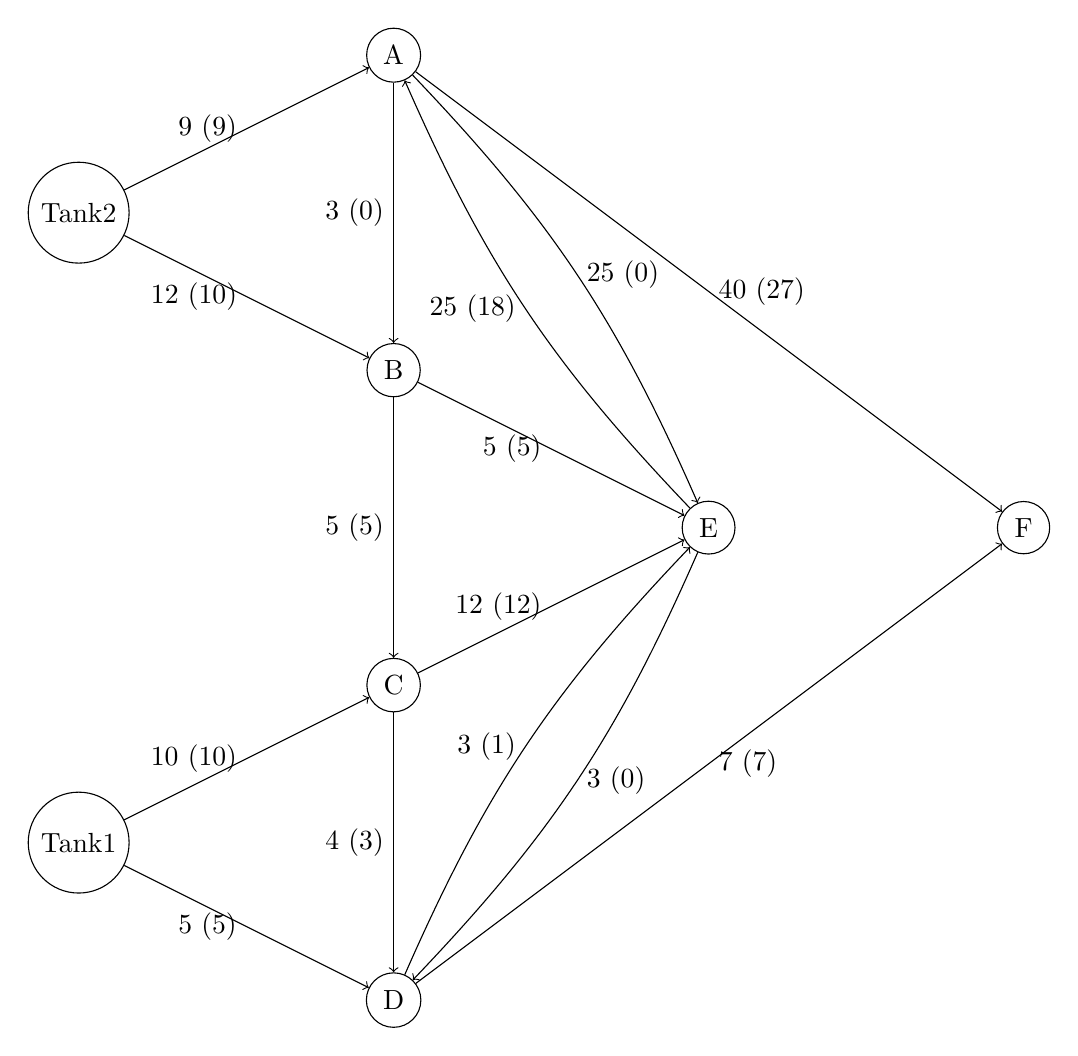
\begin{tikzpicture}
\tikzset{edge/.style = {->,> = latex'}}

\node[shape=circle,draw=black] (A) at (0,10) {Tank2};
\node[shape=circle,draw=black] (B) at (0,2) {Tank1};
\node[shape=circle,draw=black] (C) at (4,12) {A};
\node[shape=circle,draw=black] (D) at (4,8) {B};
\node[shape=circle,draw=black] (E) at (4,4) {C};
\node[shape=circle,draw=black] (F) at (4,0) {D};
\node[shape=circle,draw=black] (G) at (8,6) {E};
\node[shape=circle,draw=black] (H) at (12,6) {F};

\path [->] 

(A)	edge[] node[left] {9 (9)} (C)
(A) edge[] node[left] {12 (10)} (D)
(B) edge[] node[left] {10 (10)} (E)
(B) edge[] node[left] {5 (5)} (F)
(C) edge[] node[left] {3 (0)} (D)
(D) edge[] node[left] {5 (5)} (E)
(E) edge[] node[left] {4 (3)} (F)
(C) edge[bend left=10] node[right] {25 (0)} (G)
(G) edge[bend left=10] node[left] {25 (18)} (C)
(D) edge[] node[left] {5 (5)} (G)
(E) edge[] node[left] {12 (12)} (G)
(F) edge[bend left=10] node[left] {3 (1)} (G)
(G) edge[bend left=10] node[right] {3 (0)} (F)
(C) edge[] node[right] {40 (27)} (H)
(F) edge[] node[right] {7 (7)} (H)
;

\end{tikzpicture}

\end{question}




% --------------------------------------------------------------
%     You don't have to mess with anything below this line.
% --------------------------------------------------------------

\end{document}
